\graphicspath{{../02Physics/pics/}}
	
\chapter[Physics]{Physics}\label{ch:Physics}

\lettrine[lines=2]{\color{darkocre}N}{umbers} are powerful
mathematical objects. They are used to solve
an endless list of problems that involve \emph{quantities}. As
mathematics
and sciences progressed, natural numbers evolved into whole
numbers, then into rational numbers and beyond.\footnote{A superb account of
this process is given in the book \emph{``Number: The Language of
Science''} by Tobias Dantzig.}

At a certain stage, problems of physics needed a mathematical
tool to describe quantities with arbitrary direction. For example, a
motion of a body involves velocity -- a physical quantity describing
how fast the body is moving and in what direction. Quite rapidly
vectors led to tensors. Tensors had to be invented because there are
many important problems where tensors are very natural. Examples will
be given in the last chapter of the book.

On the surface, numbers, vectors, and tensors
are rather different. However, they have a lot in common.
Tensors are ``numbers on steroids'' in the sense that all
 things you can do with numbers, you can do with tensors, and
even more.

Before we turn to tensors, we should familiarize ourselves with
vectors. And before that, we must review the main concepts associated
with numbers.

\section{Power of Abstraction}
Mathematics is a remarkably effective and universal discipline, its
methods and
results can be applied in a wide range of fields. In part, the universality of mathematics
stems from the \emph{general} and \emph{abstract} nature of mathematical
concepts. Let us illustrate this using an example.

\begin{SCfigure}%[htbp]
  %\centering
  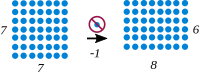
\includegraphics[scale=1.0]{numbersExampleGenerality}
  \caption{49 objects can be arranged in a square 7x7. 48 objects can
    be arranged as a rectangle of 6x8.}
  \label{fig:numbersExampleGenerality}
\end{SCfigure}

An astute farmer notices that 49 sacks of grains can be arranged
in a square with each side having 7 sacks (see the Figure
\ref{fig:numbersExampleGenerality}). When one sack is used up, the
remaining 48 sacks can be arranged as a rectangle 6 by 8 sacks.

The farmer realizes that this curious fact has nothing to do with
either grains or sacks. The same observation could be made about
buckets, chairs, people, and so on. As the first step of
generalization, the farmer states that 49 \emph{objects} can be
arranged as a 7 by 7 square, while 48 objects can be arranged
as a 6 by 8 rectangle. The farmer also notes that $48=49-1$, whereas
$6=7-1$ and $8=7+1$. She writes down the newly discovered relation as
follows:
\begin{align*}
  7*7\textrm{ obj } - 1\textrm{ obj } = (7-1) * (7+1)\textrm{ obj }\,,
\end{align*}
where \emph{obj} is the denotation of \emph{any} object.

As the grain is used up, the farmer discovers two more relations:
\begin{align*}
  6*6\textrm{ obj } - 1\textrm{ obj } = (6-1) * (6+1)\textrm{ obj }
\end{align*}
and
\begin{align*}
  5*5\textrm{ obj } - 1\textrm{ obj } = (5-1) * (5+1)\textrm{ obj }\,.
\end{align*}

At this point the farmer makes an educated guess, stating that a more
general relation must exist:
\begin{align}
  n*n - 1 = (n-1) * (n+1)\,.
  \label{eq:numbersAlgebraIdentity1}
\end{align}
In the last expression the reference to objects is dropped, the
expression is written simply in terms of \emph{numbers}.

A deeper analysis reveals that the relation given by
(\ref{eq:numbersAlgebraIdentity1}) exists for \emph{any quantities}
that obey usual rules of addition and multiplication. This includes
rational numbers, real numbers, complex numbers\index{Numbers!complex} (see Section
\ref{sec:CompoundNumbers}), and even operators! The relation
\begin{align}
  x^2-1=(x-1)(x+1)
\end{align}
 holds true because of the way we define \emph{rules for manipulation} --
 addition and multiplication in this case -- of
number-like objects, regardless of what those number-like objects
represent in a particular problem.
\begin{figure}[htbp]
  \centering
  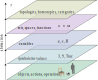
\includegraphics[scale=1.0]{numbersAbstractionLevels}
  \caption{Mathematical thinking has many levels of abstraction\index{Abstraction}. Going
    to higher levels of abstractions results in higher efficiency and
    more powerful ideas and tools.}
  \label{fig:numbersAbstractionLevels}
\end{figure}

The path from ``sacks of grain'' to a variable $x$ is the path from concrete,
specific objects to \emph{abstract} entities that are the product of
creative imagination. This path to higher levels of abstraction is
illustrated in the Figure \ref{fig:numbersAbstractionLevels}. As we
move to higher levels of abstraction, our mathematical tools become
more powerful and more universally applicable: From everyday
arithmetic, to economics, to general relativity, and quantum gravity.

Using more abstract mathematical objects requires serious mental
effort. To reach the highest levels one needs to do mathematics
professionally. However, any profession can benefit from \emph{some} level of
abstraction, and to understand vectors and tensors, we must go beyond
usual high-school level. One of the goals of this book is to help readers
build tolerance and appreciation of more abstract aspects of
mathematics.


\section{Terminology Barrier}
Every high school student has a working knowledge of bilinear operators
over associative and commutative fields\index{Field}, but hardly anyone of those
students is aware of this fact. We refer here to the ability to
simply add and multiply numbers. This demonstrates that even familiar
and basic notions may look complicated when ``dressed in unfamiliar
clothing.''

When we learn new mathematical concepts, especially at a higher level of
abstraction, we often encounter what might be called a
\emph{terminology barrier}\index{Barrier!terminology}: a concept seems
more difficult if it is
formulated in a new language, without sufficient connections to
already familiar concepts, and without clear examples of how the
concept can be applied.

New terminology is unavoidable when learning new concepts. There will
be a number of new mathematical concepts and definition introduced in
this book. To lower the terminology barrier, every new mathematical
concept will be illustrated with examples and the connections to
already familiar concepts will also be given. Additionally, it is
recommended to do the following exercise every time a new concept with
unusual terminology is introduced:

\begin{mybio}{Dealing With New Concepts}
  \begin{itemize}
    \item \phantom{x}
  \item Take a critical look at a new name and notation.
  \item Think whether the new name or notation looks like something
    you know. Is the resemblance helpful or misleading?
  \item Be creative and try to come up with your own notation or word
    to describe the new concept.
  \end{itemize}
  \vspace{0.1cm}
  \emph{Remember}: Symbols and names are not essential. What is
  important is the set of \emph{relations} of a new concept to other
  concepts. The relations show how the concept fits and functions
  within the larger framework.
\end{mybio}
Demonstrations of this approach can be found in the rest of the book.

\section{Algebra of Numbers}

We will start with the ``familiar'' numbers\index{Numbers}:
\begin{align*}
  0,\pm 1, \pm 2, \ldots, \pm n,\,\ldots
\end{align*}
This endless collection, considered as one entity, is called the
\emph{set of whole numbers}; it is denoted as $\mathbb{Z}$.

The set $\mathbb{Z}$ is not a formless heap of elements. On the
contrary, it has a rich \emph{structure}\index{Structure}. The structure of any set, including
the set of whole numbers, is
revealed through various \emph{relations}\index{Relations} between all or some of its
elements. Here are several examples:
\begin{itemize}
  \item $1$ and $-1$ are related, and so are $2$ and
    $-2$, and generally, $n$ and $-n$.
  \item Relation exists between $1$ and $2$, $2$ and $4$, $3$ and $6$,
    and generally, between $n$ and $2n$.
  \item The pairs $(1,2)$, $(2,3)$, $(3, 4$), and so on, illustrate an
    important relation of order that exists in $\mathbb{Z}$.
  \item The pairs $(2, 1)$, $(3, 1)$, $(4, 2)$, $(5, 1)$, $(6, 3)$ and
    similar ones unite a number and its greatest divisor not equal to
    the number itself.
\end{itemize}
The list can be continued indefinitely, but the general idea of
relations should be
clear. Such number-to-number relation can be schematically represented
as a box with an input and an output, as shown in the Figure
\ref{fig:schematicRelation1to1}. A few important relations are given
descriptive names: {\bf neg}, {\bf dbl}, {\bf suc}, and {\bf gsd}
are examples from the Figure \ref{fig:schematicRelation1to1}; they
correspond to negation, doubling of a number, finding the successor of
a given number, and finding the greatest divisor smaller than the
number itself.
\begin{figure}[htbp]
  \centering
  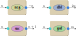
\includegraphics[scale=1.0]{schematicRelation1to1}
  \caption{Relation between elements of a set can be schematically
    represented using boxes with inputs and outputs. Here the
    relations between numbers are given descriptive names: {\bf neg}
    is negation, {\bf dbl} is doubling, {\bf suc} is getting the
    successive number, {\bf gsd} is the greatest divisor of a number smaller than
    the number itself.}
  \label{fig:schematicRelation1to1}
\end{figure}

\subsection{Functions}
What we have just described is the idea of a \emph{function}\index{Function}, or numeric
function of a single \emph{argument}\index{Argument}, to be precise. A function of a
single argument connects every \emph{argument} (input) to a certain
\emph{value} (output), establishing a \emph{relation} between a pair
of elements.
\begin{SCfigure}%[htbp]
  %\centering
  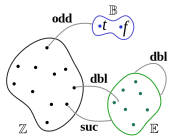
\includegraphics[scale=1.0]{diagramFunctionSingleArg}
  \caption{Relations can be viewed on the level of sets. A function
    maps (connects) one set with another in a meaningful way. For
    example, $\textrm{\bf dbl}$ maps every integer from $\mathbb{Z}$
  into the set of even numbers $\mathbb{E}$.}
  \label{fig:diagramFunctionSingleArg}
\end{SCfigure}

Another view on relations is illustrated in the Figure
\ref{fig:diagramFunctionSingleArg}. Relations between elements can be
``elevated'' to the level of sets and depicted as arrows connecting
one set (\emph{domain}) to another set (\emph{range}). Symbolically we
can write:
\[
\mathbb{Z}\overset{\textrm{\bf dbl}}{\longrightarrow} \mathbb{E}\,,
\]
where $\mathbb{E}$ denotes the set of all even numbers, {\bf dbl} is the
name of the function that doubles its argument.

The relations of the type ``one number to one number'' -- considered
above -- can be
generalized to ``several numbers to one number'' or ``one number to
several numbers'' or even ``several numbers to several numbers.'' The
schematic representation of such relations are given in the
Figure \ref{fig:schematicRelationNtoN}.
\begin{figure}[htbp]
  \centering
  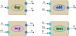
\includegraphics[scale=1.0]{schematicRelationNtoN}
  \caption{Relations of several elements to several elements:
    {\bf dup} duplicates its input, {\bf add} calculates the sum,
    {\bf swp} swaps the order of the arguments, {\bf max} returns the
    maximum of three input numbers.}
  \label{fig:schematicRelationNtoN}
\end{figure}

\begin{exercise}\label{exe:relationsGeneral}
Think how you would represent the generalized relations of the types
given in the Figure \ref{fig:schematicRelationNtoN} at the level of
sets? What kind of diagrams would you draw?
\end{exercise}

\subsubsection{Binary Functions}
An important function of two variables is the familiar {\bf add} relation:
\[
\btc{add}\,n\,m = n + m\,.
\]
The right-hand side of this equality is just another way of writing
the expression involving function with two input arguments. It is a
special case of a more general rule, which can be written as follows:
\[
f\,\,n\,m = n\circledcirc m\,.
\]
On the left we have a \emph{prefix}\index{Notation!prefix} notation, where a function $f$
is \emph{applied} to two arguments. On the right, we have an
\emph{infix}\index{Notation!infix} notation and a special symbol placed between the first
and the second argument. Several familiar examples are:
\begin{itemize}
\item $\btc{mul}\,\,n\,m = n * m$ -- multiplication.
\item $\btc{pow}\,\,n\,m = n^\wedge m$ -- power.
\item $\btc{sub}\,\,n\,m = n - m$ -- subtraction.
\item $\btc{div}\,\,n\,m = n / m$ -- division.
\end{itemize}
The functions $\btc{mul}$, $\btc{pow}$, $\btc{sub}$, and $\btc{div}$ are all examples of
\emph{binary}\index{Function!binary} functions -- functions of two arguments.
\begin{exercise}\label{exe:binaryYourOwn}
Think of a your own example of a binary function (function of two
arguments). Create its infix variant.
\end{exercise}


%\begin{tcolorbox}[colback=white!95!ocre, title=Problem]
\begin{exercise}\label{exe:ESRSymmetricAntisymmetric}
  Show that
  \[
  \epsilon_{ij}a_ia_j = 0\,.
  \]
\end{exercise}
%\end{tcolorbox}

\section*{Chapter Highlights}
{\setstretch{1.5}\chhc
  \it
  \small
\begin{itemize}
\item The power of mathematical concepts and methods increases with
  the level of abstraction.
\item Learning new concepts often involves learning new
  terminology. The latter can create an artificial mental barrier.
\item ``Usual'' numbers form a mathematical structure. The structure
  is revealed through various relations that exist between numbers.
\item Relations between numbers are expressed using the concept of
  functions and operations (e.g., addition). Each operation is
  characterized by its arity -- the number of arguments it accepts as
  an input.
\item Functions can be represented schematically as boxes with inputs
  and outputs.
\item Functions that act on natural numbers can be written using index
  notation (e.g., $f\, i = f_i$).
\item Linear functions represent the simplest but still powerful and
  useful kind of functions.
\item Functions can be composed to create new functions.
\item A function with several inputs is said to be partially applied when not
  all its inputs are populated.
\item The same function can be represented in various ways: Graphical,
  as a symbolic formula, as a table. The function is not reduced to
  any of its representations.
\item The power of abstract mathematical thinking comes, in part, from
  efficient notation. Einstein's Summation Rule (ESR) is a good
  example of this.
\end{itemize}


}
